\chapter{Architecture}
\label{sec:architecture}
\minitoc
\vspace*{1cm}

This chapter illustrates the general design of the fuzzer without getting into too much implementation details. The in-depth breakdown of the fuzzer's components is more thoroughly described in Chapter ~\ref{sec:implementation}. The key components that will be elaborated here are the high-level working view of \pname{}, instrumentation although its details are out of the scope of this thesis, 

\section{Vulnerability Detection}
\pname{} is able to detect Reflected and Stored Cross-Site Scripting(XSS) vulnerabilities, and subsequently, web applications that can be exploited for Distributed Denial of Service (DDoS) attacks. In order to detect the aforementioned vulnerabilities, we do a string-matching for the injected, possibly malicious, payload in the returned HTML response. This method may be the most efficient in terms of speed, however, it can result in high number of false positives, as the location of the payload in the response is not accounted for. False positives arise when the tool reports that an XSS was detected when in fact it was not one. One example of this would be if the XSS payload is returned enclosed with double quotes inside an HTML element's attribute. If the web application correctly escapes any double quotes found in the XSS payload then the payload will not be executable. There are plans to improve the efficiency of our XSS detection method which are discussed in Chapter ~\ref{sec:futurework}.

\section{Fuzzing Session}

\begin{figure}[ht]
 \centering
 \captionsetup{justification=centering}
 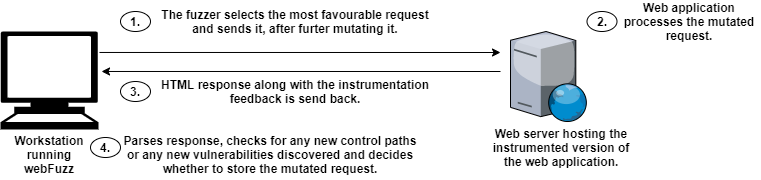
\includegraphics[width=5.0in]{figures/architecture.png}
 \caption{Simplified work process of \pname{}.}
 \label{fig:reflectedxss}
\end{figure}

% NEW SECTION
\section{Mutation}
